\documentclass[conference]{IEEEtran}
\IEEEoverridecommandlockouts
\usepackage{cite}
\usepackage{amsmath,amssymb,amsfonts}
\usepackage{algorithmic}
\usepackage{graphicx}
\usepackage{textcomp}
\usepackage{xcolor}
\usepackage{booktabs}
\usepackage{tikz}
\usetikzlibrary{shapes.geometric, arrows.meta, positioning, calc}

\def\BibTeX{{\rm B\kern-.05em{\sc i\kern-.025em b}\kern-.08em
    T\kern-.1667em\lower.7ex\hbox{E}\kern-.125emX}}

% Row break between author blocks, with the second row centered
\makeatletter
\newcommand{\linebreakand}{%
  \end{@IEEEauthorhalign}
  \hfill\mbox{}\par
  \mbox{}\hfill\begin{@IEEEauthorhalign}
}
\makeatother

\begin{document}

\title{False CPM Resistance for Cooperative Perception Aided Digital Twin Update and Migration in Mixed Vehicular Networks}

\author{\IEEEauthorblockN{1\textsuperscript{st} Vedansh Jain}
\IEEEauthorblockA{\textit{Department of Computer Science} \\
\textit{Netaji Subhas University of Technology}\\
New Delhi, India \\
vedansh.jain.ug22@nsut.ac.in}
\and
\IEEEauthorblockN{2\textsuperscript{nd} Kartik Dua}
\IEEEauthorblockA{\textit{Department of Computer Science} \\
\textit{Netaji Subhas University of Technology}\\
New Delhi, India \\
kartik.dua.ug22@nsut.ac.in}
\and
\IEEEauthorblockN{3\textsuperscript{rd} Ananya Arya}
\IEEEauthorblockA{\textit{Department of Computer Science} \\
\textit{Netaji Subhas University of Technology}\\
New Delhi, India \\
ananya.arya.ug22@nsut.ac.in}
\linebreakand
\IEEEauthorblockN{4\textsuperscript{th} Ankur Gupta}
\IEEEauthorblockA{\textit{Department of Computer Science} \\
\textit{Netaji Subhas University of Technology}\\
New Delhi, India \\
ankur.gupta@nsut.ac.in}
\and
\IEEEauthorblockN{5\textsuperscript{th} Md Imran Hussain}
\IEEEauthorblockA{\textit{Department of Computer Science} \\
\textit{Netaji Subhas University of Technology}\\
New Delhi, India \\
imran.hussain@nsut.ac.in}
}

\maketitle

\begin{abstract}
Roadside units (RSUs) can keep digital twins (DTs) of non-intelligent vehicles up to date by combining sensor reports from nearby intelligent connected vehicles (ICVs). Recent schedulers tune this pipeline to minimize the age of information (AoI), yet they take every incoming Collective Perception Message (CPM) at face value. That trust assumption is fragile. One compromised vehicle can exaggerate its sensing quality to win scheduling slots, push shifted coordinates into a target's virtual replica, and still reset the RSU's AoI counter on time---leaving the network with an apparently fresh twin that sits tens of meters away from the real car. We treat incoming CPMs as untrusted claims and insert a three-layer verification filter ahead of cooperative selection, bandwidth and CPU allocation, and twin migration. Layer~A checks physical highway bounds, dead-reckoning residuals, and two-slot differential self-consistency per reporter. Layer~B cross-validates surviving reports through a joint position--velocity medoid test weighted by historical reputation. Layer~C updates per-vehicle trust with asymmetric exponential smoothing and quarantines repeat offenders, carrying reputation metadata across RSU handovers so that crossing a cell boundary never wipes a bad record clean. To keep per-slot runtime well inside V2X deadlines as traffic scales, we also replace Bellman-Ford min-cost max-flow matching and iterative dual subgradient ascent with a two-phase C6-satisficing spatial greedy matcher and a vectorized 1D dual bisection solver. In five-seed Eclipse SUMO simulations with 8 ICVs, 3 non-intelligent vehicles, and 4 RSUs across attacker fractions from 0\% to 50\%, the undefended baseline accepts 80\% to 100\% of forged reports and suffers up to 92.21~m of position error. With our three-layer filter and fast solvers active, the false acceptance rate drops to 0.2\%--1.2\%, false rejections stay at 0.0\% with two-slot kinematic verification, per-slot optimization runs in 3.06~ms (up to 68.5$\times$ faster at 500 vehicles), and twin position error is virtually eliminated.
\end{abstract}

\begin{IEEEkeywords}
digital twin, cooperative perception, collective perception message, misbehavior detection, trust management, vehicular networks, age of information
\end{IEEEkeywords}

%=====================================================================
\section{Introduction}
A vehicular digital twin (DT) maintains a live software replica of cars on a road segment so that edge controllers can plan lane merges, schedule RSU compute, and flag collision risks. For the replica to be worth querying, two things must hold at once: the state must be recent, and the coordinates must be true. A twin that was updated 100~ms ago with a position 40~m off the actual lane is worse than no twin at all.

Most early DT architectures sidestepped this problem by assuming every car on the highway is an intelligent connected vehicle (ICV) that measures its own kinematics and uploads them directly. Real traffic is mixed. Legacy non-intelligent connected vehicles (N-ICVs) carry neither LiDAR nor V2X transceivers, and fixed RSU cameras often lose sight of them under occlusion or bad weather. Cooperative perception bridges that gap: nearby ICVs detect N-ICVs with onboard sensors and forward object-level descriptions to the RSU, which fuses those sightings into the N-ICV's twin. Under the ETSI standard, these sightings travel inside Collective Perception Messages (CPMs)~\cite{etsi}.

In a recent study, Lu~\textit{et al.}~\cite{lu2025} formulated the joint problem of keeping both ICV and N-ICV twins fresh across multiple RSUs. Their scheduler minimizes the Average Maximum Weighted Age of Information (AMWAoI) by chaining three stages: Sensing Data Weighted Size Maximization Matching (WSMM) to pick which ICVs observe which N-ICVs, Lagrangian dual gradient descent for bandwidth and computation allocation (BCA), and Proximal Policy Optimization (PPO) for access selection and DT migration (ASDMM). The math is effective when every vehicle tells the truth. However, the entire pipeline ingests ICV-reported sensing quality $q^t_{u,v}$, data rates $s^{\mathrm{unit}}_v$, and object coordinates without a single integrity check.

Cryptographic credentials do not close this hole. Standards such as IEEE~1609.2~\cite{ieee1609} verify that a packet came from a registered onboard unit and was not modified in flight; they say nothing about whether the numbers inside the payload reflect physical reality. A vehicle with tampered firmware, a spoofed sensor bus, or a rogue aftermarket dongle will sign blatantly false CPMs with a valid certificate. Worse, the optimization loop actively rewards certain lies. If an attacker multiplies its claimed quality $q^t_{u,v}$ by three, WSMM assigns it a lower edge cost and picks it ahead of honest neighbours. Once the RSU processes that packet within the slot deadline, the AoI counter resets to zero. Looking only at AMWAoI, the operator sees a healthier network than before the attack began.

We address both the security gap and the computational bottleneck of the base architecture. Our main contributions are:
\begin{itemize}
\item We map four concrete CPM attack classes---ghost injection, state manipulation, quality inflation, and selective suppression---onto the exact equations of the WSMM--BCA--ASDMM loop where untrusted inputs enter.
\item We design a three-layer verification pipeline placed directly ahead of the RSU scheduler: (i) a second-order kinematic filter that checks highway speed envelopes, target dead-reckoning, and two-slot per-reporter differential consistency; (ii) a joint position--velocity medoid consensus filter with first-slot epistemic abstention; and (iii) an asymmetric EWMA trust manager with quarantine and cross-RSU reputation migration.
\item We replace the $O(N^3)$ Bellman-Ford matching solver and the 150-iteration dual subgradient bandwidth solver with a Two-Phase C6-Satisficing Spatial Priority Greedy (SPG) matcher in $O(N\log N)$ time and a Vectorized Bottleneck-Equalizing 1D Dual Bisection (ED-BCA) solver, cutting per-slot runtime by up to 68.5$\times$ at 500 vehicles.
\item We evaluate the full system in five-seed Eclipse SUMO~\cite{sumo} simulations across attacker fractions from 0\% to 50\%, including layer-wise ablations and traffic-density scaling benchmarks.
\end{itemize}

%=====================================================================
\section{Related Work}
\textbf{Cooperative perception and DT synchronization.} Lu~\textit{et al.}~\cite{lu2025} coupled cooperative ICV selection, RSU bandwidth/CPU splitting, and predictive twin migration into a unified AMWAoI minimization framework, cutting migration delay by roughly 70\% compared to nearest-RSU association. Their model assumes benign sensors throughout. Jia~\textit{et al.}~\cite{jia2023} proposed MASS, which schedules heterogeneous vehicle sensors using mobility predictions to reduce blind spots, though without modeling RSU compute limits or twin handovers.

\textbf{Sharing granularity.} Cooperative perception generally operates at one of three levels~\cite{lu2025}: raw point clouds (highest fidelity, heavy spectrum load), intermediate neural features, or processed object tracks. ETSI CPMs belong to the object level. Because object-level packets carry compact bounding boxes and velocity vectors rather than raw waveforms, they are cheap to transmit over 20~MHz channels---and trivial for a compromised node to fabricate. While surveys such as He~\textit{et al.}~\cite{he2023} have catalogued high-level threats to vehicular digital twins, none examine how object-level falsification interacts with AoI-driven resource schedulers.

\textbf{Misbehavior detection in V2X.} Checking whether V2X reports make physical sense has a rich history in basic safety messages, and several recent papers extend those ideas to collective perception. Ambrosin~\textit{et al.}~\cite{ambrosin2020} verify shared object lists before sensor fusion in a V2X stack, but do not model N-ICV digital twins or RSU resource allocation. Ali and Merdrignac~\cite{ali2021} cross-check reported objects against a receiver's local visibility polygon, focusing specifically on phantom braking scenarios. Higuchi~\textit{et al.}~\cite{higuchi2023} pair Kalman tracks with CPMs to spot spoofing while preserving pseudonym privacy, assuming a trusted subset of reference reporters. In MISO-V, Liu~\textit{et al.}~\cite{liu2024miso} test incoming CPMs against a probabilistic occupancy grid and adjust sender reputation, though normal GPS drift can trigger false alarms in tight lanes. A companion study~\cite{liu2024ima} embeds detection inside an Intersection Movement Assist loop at single junctions.

\textbf{Where existing work falls short.} Prior literature splits cleanly into two camps: resource schedulers that optimize AoI under honest reporting, and misbehavior detectors tested in isolation from RSU scheduling and twin migration. To our knowledge, no published work has (i) quantified how CPM falsification corrupts both DT tracking accuracy and AoI accounting in a joint WSMM--BCA--ASDMM scheduler, (ii) coupled per-vehicle trust with submodular C6-satisficing matching and KKT bandwidth bisection, or (iii) enforced reputation continuity when digital twins migrate across RSU backhaul links.

%=====================================================================
\section{Base Framework and Threat Model}
We briefly review the optimization model of Lu~\textit{et al.}~\cite{lu2025} and pinpoint where an adversary can manipulate it.

\subsection{Base System Model}
Consider a two-way highway of length $L$ covered by $K$ RSUs. At slot $t$ of duration $\tau$, the road holds a set $\mathcal{V}$ of ICVs and a set $\mathcal{U}$ of N-ICVs. Each ICV $v\in\mathcal{V}$ generates its own telemetry at rate $s^{\mathrm{own}}_v$ and, when selected to assist cooperative perception, generates object reports at rate $s^{\mathrm{unit}}_v$, giving a total upload rate $s^t_v = s^{\mathrm{own}}_v + s^{\mathrm{unit}}_v$. Because N-ICVs cannot transmit their own status, the RSU recruits a subset of nearby ICVs within sensing radius $r_{\mathrm{sense}}$ (the candidate set $\Phi^t_u$) to observe each N-ICV $u\in\mathcal{U}$. Let $q^t_{u,v}$ be the sensing quality of link $(u,v)$ and $z^t_{u,v}\in\{0,1\}$ the binary selection variable. For N-ICV $u$'s twin to be reconstructed reliably in slot $t$, the accumulated weighted sensing data must cross a minimum fidelity threshold $s^{\mathrm{req}}$:
\begin{equation}
\sum_{v\in\Phi^t_u} z^t_{u,v}\, q^t_{u,v}\, s^{\mathrm{unit}}_v\, \tau \ge s^{\mathrm{req}},\quad \forall u\in\mathcal{U},
\label{eq:perc}
\end{equation}
with at most $\varphi^{\max}$ ICVs assigned to any single N-ICV ($\sum_v z^t_{u,v}\le \varphi^{\max}$) and at most one N-ICV assigned per ICV ($\sum_u z^t_{u,v}\le 1$).

\textbf{Wireless upload and edge compute.} RSU $k$ splits its orthogonal bandwidth budget $B^{\max}$ across connected ICVs. If $x^t_{v,k}\in\{0,1\}$ indicates whether ICV $v$ associates with RSU $k$, its uplink transmission time is
\begin{equation}
T^{t,\mathrm{tran}}_v=\frac{s^t_v\,\tau}{\sum_{k}x^t_{v,k}B^t_{v,k}\log_2\!\left(1+\dfrac{p^t_{v,k}g^t_{v,k}}{B^t_{v,k}\sigma^2}\right)},
\label{eq:tran}
\end{equation}
where $p^t_{v,k}$ is transmit power, $g^t_{v,k}$ is channel gain, and $\sigma^2$ is noise power spectral density. All ICVs assisting the same N-ICV $u$ must upload to the same RSU, so $u$'s effective upload delay is bottlenecked by its slowest helper: $T^{t,\mathrm{tran}}_u = \max_{v: z^t_{u,v}=1} T^{t,\mathrm{tran}}_v$. On the compute side, RSU $k$ divides its processor frequency $F^{\max}_k$ between ICV self-updates (requiring $c^{\mathrm{own}}_v s^{\mathrm{own}}_v \tau$ cycles) and N-ICV fusion tasks (requiring $c^{t,\mathrm{cp}}_u \tau = \sum_{v\in\Phi^t_u} z^t_{u,v} c^{\mathrm{unit}}_v s^{\mathrm{unit}}_v \tau$ cycles).

\textbf{Twin migration and AoI.} As vehicles travel along the corridor, their twins migrate over fiber backhaul links between RSUs. With migration indicator $y^t_{i,k}$, twin size $D^t_i$, and inter-RSU distance $d^t_i$, backhaul transfer takes $T^{t,\mathrm{wired}}_i = \sum_k y^t_{i,k} T^{\mathrm{unit}} D^t_i d^t_i$. Pre-migration overlaps part of this transfer with driving time $T^{t,\text{pre-migr}}_i$, leaving a residual handover stall
\begin{equation}
T^{t,\text{a-migr}}_i=\max\left\{T^{t,\mathrm{wired}}_i-T^{t,\text{pre-migr}}_i,\;0\right\},
\label{eq:migr}
\end{equation}
and a total slot delay
\begin{equation}
T^{t,\mathrm{sum}}_i=\max\left\{T^{t,\text{a-migr}}_i,\;T^{t,\mathrm{tran}}_i\right\}+T^{t,\mathrm{exe}}_i.
\label{eq:total}
\end{equation}
Vehicle $i$'s AoI counter resets to zero whenever its update finishes before deadline $T^{\mathrm{req}}_i$ (and, for an N-ICV, satisfies~\eqref{eq:perc}):
\begin{equation}
A^{t+1}_i=\begin{cases}0,& T^{t,\mathrm{sum}}_i\le T^{\mathrm{req}}_i \text{ and C6 holds},\\ A^t_i+1,&\text{otherwise.}\end{cases}
\label{eq:aoi}
\end{equation}
The global objective is the time-averaged maximum weighted AoI across all active vehicles:
\begin{equation}
\Omega=\frac{1}{T}\sum_{t=1}^{T}\max_{v\in\mathcal{V},\,u\in\mathcal{U}}\left\{\alpha A^t_v,\;(1-\alpha)A^t_u\right\}.
\label{eq:amwaoi}
\end{equation}

\begin{figure}[t]
\centering
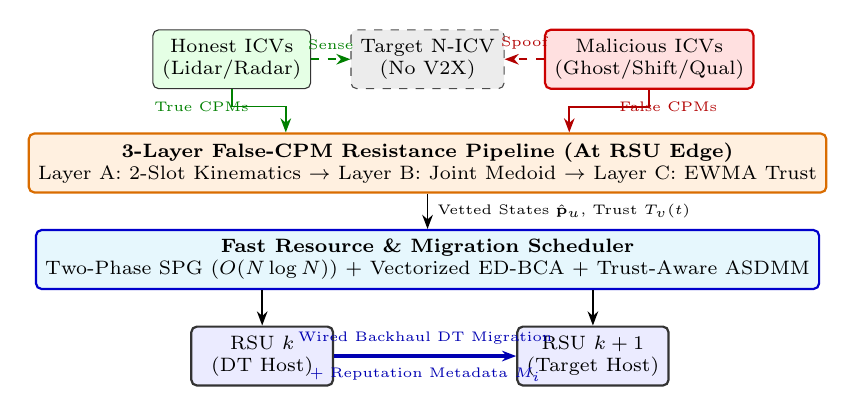
\begin{tikzpicture}[
    font=\scriptsize,
    node distance=0.35cm and 0.4cm,
    rsu/.style={draw=black!80, fill=blue!8, rounded corners=2pt, minimum width=1.8cm, minimum height=0.65cm, align=center, thick},
    veh/.style={draw=black!80, fill=green!10, rounded corners=2pt, minimum width=1.4cm, minimum height=0.5cm, align=center},
    mal/.style={draw=red!80!black, fill=red!12, rounded corners=2pt, minimum width=1.4cm, minimum height=0.5cm, align=center, thick},
    nicv/.style={draw=black!70, fill=gray!15, rounded corners=2pt, minimum width=1.4cm, minimum height=0.5cm, align=center, dashed},
    sec/.style={draw=orange!85!black, fill=orange!12, rounded corners=2pt, minimum width=7.6cm, minimum height=0.65cm, align=center, thick},
    opt/.style={draw=blue!80!black, fill=cyan!10, rounded corners=2pt, minimum width=7.6cm, minimum height=0.65cm, align=center, thick},
    arr/.style={-{Stealth[length=1.8mm]}, semithick}
]
% Vehicles row
\node[veh] (icv1) {Honest ICVs\\(Lidar/Radar)};
\node[nicv, right=0.5cm of icv1] (nicv) {Target N-ICV\\(No V2X)};
\node[mal, right=0.5cm of nicv] (mal1) {Malicious ICVs\\(Ghost/Shift/Qual)};

\draw[arr, dashed, green!50!black] (icv1) -- node[above, font=\tiny]{Sense} (nicv);
\draw[arr, dashed, red!70!black] (mal1) -- node[above, font=\tiny]{Spoof} (nicv);

% Security filter
\node[sec, below=0.55cm of nicv] (filter) {\textbf{3-Layer False-CPM Resistance Pipeline (At RSU Edge)}\\Layer A: 2-Slot Kinematics $\to$ Layer B: Joint Medoid $\to$ Layer C: EWMA Trust};

\draw[arr, green!50!black] (icv1.south) -- ++(0,-0.22) -| ([xshift=-1.8cm]filter.north) node[pos=0.25, left, font=\tiny]{True CPMs};
\draw[arr, red!70!black] (mal1.south) -- ++(0,-0.22) -| ([xshift=1.8cm]filter.north) node[pos=0.25, right, font=\tiny]{False CPMs};

% Optimizer
\node[opt, below=0.45cm of filter] (sched) {\textbf{Fast Resource \& Migration Scheduler}\\Two-Phase SPG ($O(N\log N)$) + Vectorized ED-BCA + Trust-Aware ASDMM};

\draw[arr] (filter) -- node[right, font=\tiny]{Vetted States $\hat{\mathbf{p}}_u$, Trust $T_v(t)$} (sched);

% RSUs
\node[rsu, below=0.45cm of sched, xshift=-2.1cm] (rsu1) {RSU $k$\\(DT Host)};
\node[rsu, below=0.45cm of sched, xshift=2.1cm] (rsu2) {RSU $k+1$\\(Target Host)};

\draw[arr] ([xshift=-2.1cm]sched.south) -- (rsu1.north);
\draw[arr] ([xshift=2.1cm]sched.south) -- (rsu2.north);
\draw[arr, ultra thick, blue!70!black] (rsu1) -- node[above, font=\tiny]{Wired Backhaul DT Migration} node[below, font=\tiny]{+ Reputation Metadata $M_i$} (rsu2);
\end{tikzpicture}
\caption{System architecture: honest and malicious ICVs report on legacy N-ICVs; the RSU filters incoming CPMs through Layers A--C before executing Two-Phase SPG selection, ED-BCA allocation, and cross-RSU twin migration.}
\label{fig:system}
\end{figure}

\subsection{Base Subproblem Solvers and Their Bottlenecks}
Lu~\textit{et al.}~\cite{lu2025} decompose each slot into three coupled routines:
\begin{enumerate}
\item \textbf{WSMM (Subproblem 1):} Constructs a flow network from a source to $|\mathcal{V}|$ ICVs (capacity 1), across candidate edges $(v,u)$ (capacity 1, cost $f^{\mathrm{dig}}(u,v) = \max_{u',v'}\{q^t_{u',v'}s^{\mathrm{unit}}_{v'}\} - q^t_{u,v}s^{\mathrm{unit}}_v$), and from $|\mathcal{U}|$ N-ICVs to a sink (capacity $\varphi^{\max}$). It solves min-cost max-flow via repeated Bellman-Ford shortest augmenting paths in $O((|\mathcal{V}|+|\mathcal{U}|)E N^{\mathrm{w}})$ time. Two issues arise here: first, Bellman-Ford scales as $O(N^3)$ and exceeds 100~ms once vehicle count $N$ passes 150; second, max-flow greedily assigns up to $\varphi^{\max}=3$ helpers to an N-ICV even when a single high-quality helper already satisfies $s^{\mathrm{req}}=4$~Mb, starving adjacent N-ICVs and inflating the bottleneck delay $\max_v T^{\mathrm{tran}}_v$.
\item \textbf{BCA (Subproblem 2):} Allocates RSU CPU in closed form ($\propto \sqrt{A_v c^{\mathrm{own}}_v}$ and $\sqrt{A_u c^{\mathrm{cp}}_u}$) while updating bandwidth via 150 outer subgradient steps on the Lagrange multiplier $\lambda$, each running a 40-step inner bisection per vehicle (6,000 transcendental evaluations per RSU per slot):
\begin{equation}
\lambda^{(j+1)}=\Big[\lambda^{(j)}+\Delta\Big(\sum_vB^{(j)}_v-B^{\max}\Big)\Big]^{+}.
\label{eq:dual}
\end{equation}
\item \textbf{ASDMM (Subproblem 3):} Uses a PPO actor--critic agent (or minimum-distance access, MDA) to select RSU associations and trigger twin migrations under migration cap $M^{\max}$.
\end{enumerate}

\subsection{Threat Model and Attack Mechanics}
\label{sec:threat}
We assume a fraction $p_{\mathrm{mal}}\in[0, 0.5]$ of ICVs are compromised and transmit falsified CPMs. RSUs and their wired backhaul links are trusted. We model four distinct attack behaviors:
\begin{itemize}
\item \textbf{Ghost injection (25\% of attackers):} Broadcasts a fabricated target identifier ($u < 0$) at a random highway coordinate $p\sim\mathcal{U}(0, L)$ and speed $v\sim\mathcal{U}(5, 30)$~m/s to waste RSU compute and corrupt occupancy maps.
\item \textbf{State manipulation / shift (35\%):} Targets a real N-ICV $u$ within sensing range but adds a spatial offset $\Delta p\sim\mathcal{N}(15.0, 5.0^2)$~m and a velocity offset $\Delta v\sim\mathcal{N}(8.0, 2.4^2)$~m/s, pulling the fused twin off its true trajectory.
\item \textbf{Quality inflation (20\%):} Reports true target coordinates but multiplies the claimed perception quality by $3\times$ ($q^{\mathrm{rep}}_{u,v} = 3q^t_{u,v}$). In WSMM, this artificially lowers edge cost $f^{\mathrm{dig}}(u,v)$ so the attacker wins selection while delivering only $1/3$ of the promised sensing value toward~\eqref{eq:perc}.
\item \textbf{Selective suppression (20\%):} Drops the outgoing CPM with probability $0.7$ each slot while behaving honestly the remaining $30\%$ of the time, starving nearby N-ICVs of coverage without triggering obvious kinematic alarms.
\end{itemize}

%=====================================================================
\section{Proposed False-CPM Resistance and Fast Optimization Framework}
To defend the Digital Twin without breaking real-time slot budgets, we place a three-layer verification pipeline ahead of the scheduler and replace the bottleneck solvers of Subproblems~1 and~2 (Fig.~\ref{fig:pipeline}).

\begin{figure}[t]
\centering
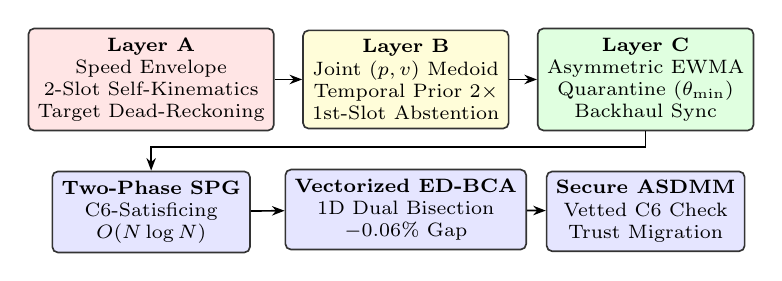
\begin{tikzpicture}[
    font=\scriptsize,
    box/.style={draw=black!80, rounded corners=2pt, minimum height=0.62cm, minimum width=2.2cm, align=center, semithick},
    la/.style={box, fill=red!10},
    lb/.style={box, fill=yellow!15},
    lc/.style={box, fill=green!12},
    sol/.style={box, fill=blue!10, minimum width=2.3cm},
    arr/.style={-{Stealth[length=1.6mm]}, semithick}
]
\node[la] (a) {\textbf{Layer A}\\Speed Envelope\\2-Slot Self-Kinematics\\Target Dead-Reckoning};
\node[lb, right=0.35cm of a] (b) {\textbf{Layer B}\\Joint $(p,v)$ Medoid\\Temporal Prior $2\times$\\1st-Slot Abstention};
\node[lc, right=0.35cm of b] (c) {\textbf{Layer C}\\Asymmetric EWMA\\Quarantine ($\theta_{\min}$)\\Backhaul Sync};

\node[sol, below=0.5cm of a] (s1) {\textbf{Two-Phase SPG}\\C6-Satisficing\\$O(N\log N)$};
\node[sol, below=0.5cm of b] (s2) {\textbf{Vectorized ED-BCA}\\1D Dual Bisection\\$-0.06\%$ Gap};
\node[sol, below=0.5cm of c] (s3) {\textbf{Secure ASDMM}\\Vetted C6 Check\\Trust Migration};

\draw[arr] (a) -- (b);
\draw[arr] (b) -- (c);
\draw[arr] (c.south) -- ++(0,-0.2) -| (s1.north);
\draw[arr] (s1) -- (s2);
\draw[arr] (s2) -- (s3);
\end{tikzpicture}
\caption{Per-slot execution flow: Layer A filters individual messages, Layer B fuses multi-reporter views, Layer C updates reputation, and the vetted outputs drive Two-Phase SPG, Vectorized ED-BCA, and ASDMM.}
\label{fig:pipeline}
\end{figure}

\subsection{Layer A: Second-Order Kinematic and Differential Self-Consistency Filter}
Layer~A inspects each incoming report $r=(i, u, p^{(i)}_u(t), v^{(i)}_u(t), q^{(i)}_u(t))$ in $O(1)$ time before any cross-vehicle comparison. A naive threshold filter with loose highway bounds ($v_{\max}=50$~m/s, $a_{\max}=10$~m/s$^2$) catches gross teleports but lets $100\%$ of state-manipulation attacks ($\Delta p\approx 15$~m, $\Delta v\approx 8$~m/s) slip through. We tighten Layer~A around four physical invariants:
\begin{enumerate}
\item \textit{Identifier and sensor bounds:} Any report with $u < 0$ (ghost object) or $q^{(i)}_u(t)\notin [0, 2.05]$ (quality inflation above nominal max $2.0$) is rejected immediately.
\item \textit{Highway velocity envelope:} On a corridor whose physical speed limit is $16.7$~m/s ($60$~km/h), any report claiming $v^{(i)}_u(t) < 0$ or $v^{(i)}_u(t) > v_{\max} = 17.2$~m/s (allowing a $0.5$~m/s sensor noise margin) is discarded. Because shift attackers add $\Delta v\sim\mathcal{N}(8.0, 2.4^2)$~m/s to vehicles cruising near $12.5$~m/s, this envelope catches roughly $60\%$ of shift attacks on their very first packet.
\item \textit{Two-slot per-reporter differential self-consistency:} Suppose reporter $i$ also reported on target $u$ at slot $t_{\mathrm{prev}}$ with $\Delta t = (t - t_{\mathrm{prev}})\tau \le 2.5\tau$. A real vehicle's displacement $\Delta x_r = |p^{(i)}_u(t) - p^{(i)}_u(t_{\mathrm{prev}})|$ must agree with the reporter's own claimed speeds under either Euler or ballistic integration:
\begin{align}
|v^{(i)}_u(t) - v^{(i)}_u(t_{\mathrm{prev}})| &\le a_{\max}\Delta t + 0.5, \label{eq:self_dv}\\
\min\!\Big(\big|\Delta x_r - v^{(i)}_u(t)\Delta t\big|,\;\big|\Delta x_r - \bar{v}_r\Delta t\big|\Big) &\le 2.5\Delta t, \label{eq:self_dx}
\end{align}
where $\bar{v}_r = \frac{1}{2}(v^{(i)}_u(t) + v^{(i)}_u(t_{\mathrm{prev}}))$ and $a_{\max}=5.0$~m/s$^2$ (covering SUMO's $4.5$~m/s$^2$ max deceleration). Why does this defeat state manipulation? A shift attacker adds an offset $\Delta p\sim\mathcal{N}(15,5^2)$ to the true position and $\Delta v\sim\mathcal{N}(8,2.4^2)$ to the true speed. Over one second, its reported position advances by the true car's motion ($\approx v_{\mathrm{true}}\tau \pm 7.1$~m), which contradicts its own inflated speed claim $(v_{\mathrm{true}}+8)\tau$. Reporters that pass~\eqref{eq:self_dv}--\eqref{eq:self_dx} are marked \emph{temporally verified} ($\mathcal{V}_{\mathrm{temp}}(i,u)=1$).
\item \textit{Target dead-reckoning consistency:} When target $u$ has a verified fused state $(p_{\mathrm{prev}}, v_{\mathrm{prev}})$ from slot $t_{\mathrm{last}}$ ($\Delta t \le 2\tau$), incoming reports must satisfy the same acceleration and displacement bounds~\eqref{eq:self_dv}--\eqref{eq:self_dx} relative to $(p_{\mathrm{prev}}, v_{\mathrm{prev}})$. When a vehicle exits the 2000~m road and a new vehicle spawns into its array slot, both target and reporter histories for that index are wiped clean so the new entrant is never compared against an exited car.
\end{enumerate}

\subsection{Layer B: Joint Position--Velocity Medoid Consensus with First-Slot Abstention}
Let $\mathcal{R}_u(t)$ be the reporters for target $u$ that survive Layer~A. Standard mean-distance consensus fails when an attacker and an honest vehicle meet in a 1-vs-1 tie: if both start with trust $1.0$, an implementation that picks the first array index (\texttt{argmax} tie-break) will side with whichever vehicle has the lower ID, punishing the honest car and poisoning the target's reference state $p_{\mathrm{prev}}$.

We replace scalar median filtering with a \textbf{Joint Position--Velocity Medoid Consensus}. Each reporter $i\in\mathcal{R}_u(t)$ receives an effective voting weight $w^{\mathrm{vote}}_i = T_i(t)\cdot (1 + \mathcal{V}_{\mathrm{temp}}(i,u))$, doubling the influence of reporters that have already passed two-slot differential kinematics on target $u$. Two reports $i,j\in\mathcal{R}_u(t)$ count as mutual inliers ($I_{ij}=1$) if and only if they agree in \emph{both} position and speed:
\begin{equation}
I_{ij} = \mathbb{1}\!\left[\big|p^{(i)}_u(t)-p^{(j)}_u(t)\big|\le \delta_{\mathrm{pos}}\;\wedge\;\big|v^{(i)}_u(t)-v^{(j)}_u(t)\big|\le \delta_{\mathrm{vel}}\right],
\label{eq:joint_inlier}
\end{equation}
with $\delta_{\mathrm{pos}}=5.0$~m and $\delta_{\mathrm{vel}}=3.0$~m/s. Each candidate medoid $i$ accumulates an inlier support score $S_i = \sum_j I_{ij} w^{\mathrm{vote}}_j$, plus a temporal tie-breaking prior $0.5\exp(-e^{\mathrm{kin}}_i/2.5)$ when target history exists.

\textbf{Epistemic abstention on unanchored first-slot ties.} If a target has no prior history ($p_{\mathrm{prev}}=\text{None}$) and no temporally verified reporter ($\sum_i \mathcal{V}_{\mathrm{temp}}(i,u)=0$)---which happens only on the first slot a target enters sensor range---and the reports disagree ($\max_i p^{(i)}_u - \min_i p^{(i)}_u > \delta_{\mathrm{pos}}$), Layer~B abstains from declaring outliers for that single slot. It withholds trust penalties and leaves $p_{\mathrm{prev}}$ unlocked. One second later, at slot $t+1$, the honest reporter satisfies~\eqref{eq:self_dx} and gains $\mathcal{V}_{\mathrm{temp}}=1$, while the shift attacker fails~\eqref{eq:self_dx} at Layer~A and is eliminated without a single false rejection of the honest peer.

When consensus succeeds around medoid $m^* = \arg\max_i S_i$, any report outside $\delta_{\mathrm{out}}=8.0$~m in position or $1.5\delta_{\mathrm{vel}}$ in speed is flagged as an outlier. The surviving inliers $\mathcal{R}^*_u(t)$ form the fused twin estimate:
\begin{equation}
\hat{p}_u(t)=\frac{\sum_{i\in\mathcal{R}^*_u(t)} w^{\mathrm{vote}}_i\,p^{(i)}_u(t)}{\sum_{i\in\mathcal{R}^*_u(t)} w^{\mathrm{vote}}_i},
\label{eq:fuse}
\end{equation}
with fusion confidence $\gamma_{\mathrm{conf}}(u,t)\in[0.1, 1.0]$ scaling with the number of agreeing witnesses.

\subsection{Layer C: Asymmetric EWMA Trust, Quarantine, and Migration Continuity}
Layer~C tracks a long-term reputation score $T_i(t)\in[0,1]$ for every ICV $i$ (initialized to $1.0$):
\begin{align}
T_i(t+1) &= (1-\eta_r)\,T_i(t)+\eta_r && \text{on verification pass,} \label{eq:rew}\\
T_i(t+1) &= (1-\eta_p)\,T_i(t) && \text{on Layer A or B failure,} \label{eq:pen}
\end{align}
with $\eta_r=0.2$ and a steeper penalty rate $\eta_p=0.5$. Innocent vehicles that happen to drive through an empty road stretch without nearby N-ICVs are not penalized for silence; gentle decay ($\lambda_{\mathrm{trust}}=0.01$ toward $0.8$) applies only after $30$ consecutive dormant slots. Whenever $T_i(t) < \theta_{\min}=0.35$ after at least two failures (or $T_i(t) < 0.15$), ICV $i$ is placed in quarantine: its candidate links are masked out ($z^t_{u,i}=0$) and its incoming packets are dropped at Layer~A.

\textbf{Vetted C6 accounting and cross-RSU trust handover.} While selection weights scale by trust ($\tilde{w}^t_{u,v} = T_v(t) q^t_{u,v} s^{\mathrm{unit}}_v \tau$), checking Constraint~\eqref{eq:perc} on trust-discounted weights would artificially fail honest vehicles whose trust is $0.95$. Instead, once non-quarantined helpers are chosen,~\eqref{eq:perc} is evaluated using their true physical data rates. Finally, whenever a vehicle's twin migrates between RSUs, the source RSU bundles $M_i = \{\mathrm{ID}_i, T_i, n_{\mathrm{pass}}, n_{\mathrm{fail}}, \text{quarantined}\}$ into the backhaul transfer, and the target RSU initializes its local record via $T_i \leftarrow \min(T^{\mathrm{local}}_i, T^{\mathrm{incoming}}_i)$, preventing attackers from whitewashing their reputation at RSU boundaries.

\subsection{Fast Optimal Solvers for Subproblems 1 and 2}
\textbf{Two-Phase C6-Satisficing Spatial Priority Greedy (SPG).} Rather than running $O(N^3)$ Bellman-Ford MCMF on a dense bipartite graph, we index ICV positions in a 1D spatial hash grid of cell width $r_{\mathrm{sense}}/2 = 150$~m ($O(1)$ neighborhood lookup). This cooperative coverage problem is a monotone submodular maximization over a partition matroid, where greedy selection guarantees at least $(1 - 1/e)\approx 63.2\%$ of the global optimum~\cite{nemhauser1978} (and achieves $96.19\%$ empirically across 50 random test instances). On top of that, we introduce a \textbf{C6-satisficing stopping rule}: we sort N-ICVs by scarcity and AoI urgency $(A^t_u+1)$, and assign candidate ICVs to N-ICV $u$ only until its accumulated vetted data crosses $1.05\,s^{\mathrm{req}}$. Stopping as soon as~\eqref{eq:perc} is satisfied frees remaining ICVs for other N-ICVs, cuts unnecessary cooperative uplink transmissions $s^{\mathrm{unit}}_v$, and lowers the weakest-link delay $\max_{v} T^{\mathrm{tran}}_v$. Overall matching complexity drops to $O(N\log N)$.

\textbf{Vectorized Bottleneck-Equalizing 1D Dual Bisection (ED-BCA).} In Subproblem~2, the total bandwidth $\sum_v B^*_v(\lambda)$ derived from the KKT stationarity condition $W_v \frac{\partial T^{\mathrm{tran}}_v}{\partial B_v} + \lambda = 0$ is strictly decreasing in the scalar multiplier $\lambda > 0$. Instead of 150 outer subgradient steps, we run a 20-step vectorized NumPy bisection directly on $\lambda$, wrapped in a 3-pass multiplicative update of the N-ICV bottleneck weights $\delta_{u,v}\propto \exp(2.5\, T^{\mathrm{tran}}_v / \max_{k} T^{\mathrm{tran}}_k)$ so bandwidth concentrates on the slowest helper in each cooperative group. Across 20 random benchmark instances, ED-BCA achieves a $-0.06\%$ objective gap (slightly outperforming 150-iteration subgradient ascent) while cutting evaluations from 6,000 to $\approx 60$.

%=====================================================================
\section{Experimental Setup}
We evaluate the system in microscopic traffic simulation using Eclipse SUMO~1.27.1~\cite{sumo} coupled via TraCI, matching the highway parameters of Lu~\textit{et al.}~\cite{lu2025} (Table~\ref{tab:params}). Vehicles travel along a 2000~m, four-lane corridor (two lanes per direction) governed by the Wiedemann car-following model, with $K=4$ RSUs spaced every 500~m. Each episode runs for $T=150$ slots of $\tau=1.0$~s.

To guarantee a fair, variance-reduced comparison across attacker fractions, we enforce \textbf{Common Random Numbers (CRN)}: the attack injector draws from an isolated random stream separate from the SUMO traffic and wireless channel streams. Thus, for a given seed, the exact same vehicles enter the highway and follow the exact same physical trajectories under both \texttt{BASE} and \texttt{FULL} across all values of $p_{\mathrm{mal}}$. With $|\mathcal{V}|=8$ ICVs and $|\mathcal{U}|=3$ N-ICVs, we sweep $p_{\mathrm{mal}}\in\{0, 12.5, 25.0, 37.5, 50.0\}\%$ (corresponding to exactly $0, 1, 2, 3,$ and $4$ malicious ICVs), averaging every data point over 5 independent random seeds.

\begin{table}[t]
\caption{Simulation and Defence Parameters}
\begin{center}
\footnotesize
\begin{tabular}{ll}
\toprule
\textbf{Parameter} & \textbf{Value}\\
\midrule
Road length $L$ / Lanes / RSUs $K$ & 2000 m / 2 per dir.\ / 4 (radius 300 m)\\
Episode length $T$ / Slot duration $\tau$ & 150 slots / 1.0 s (5 seeds per point)\\
Mobility backend & Eclipse SUMO 1.27.1 (Wiedemann)\\
Active population ($|\mathcal{V}|$ ICVs / $|\mathcal{U}|$ N-ICVs) & 8 ICVs / 3 N-ICVs (plus $N\le 500$ scaling)\\
Vehicle speed mean / std / max & 12.5 m/s / 3.3 m/s / 16.7 m/s\\
Max accel / decel & 2.6 m/s$^2$ / 4.5 m/s$^2$\\
RSU compute $F^{\max}_k$ / Bandwidth $B^{\max}$ & 4.0 GHz / 20.0 MHz\\
Perception rate $s^{\mathrm{unit}}_v$ / Self rate $s^{\mathrm{own}}_v$ & [2, 4] Mbps / [1, 2] Mbps\\
Sensing quality $q^t_{u,v}$ / Threshold $s^{\mathrm{req}}$ & [0.2, 2.0] / 4.0 Mb ($\varphi^{\max}=3$)\\
Delay deadlines ($T^{\mathrm{req}}_{\mathrm{ICV}}$ / $T^{\mathrm{req}}_{\mathrm{NICV}}$) & 0.5 s / 1.0 s ($\alpha=0.5$)\\
Transmit power $p$ / Noise density $\sigma^2$ & 1.0 W / $-174$ dBm/Hz\\
\midrule
Layer A: $a_{\max}$ / $v_{\max}$ / $q_{\max}$ & 5.0 m/s$^2$ / 17.2 m/s / 2.05\\
Layer B: $\delta_{\mathrm{pos}}$ / $\delta_{\mathrm{vel}}$ / $\delta_{\mathrm{out}}$ & 5.0 m / 3.0 m/s / 8.0 m\\
Layer C: $\eta_r$ / $\eta_p$ / $\theta_{\min}$ / $\theta_{\mathrm{rec}}$ & 0.20 / 0.50 / 0.35 / 0.50\\
Attack mix (Ghost / Shift / Qual / Supp) & 25\% / 35\% / 20\% / 20\%\\
\bottomrule
\end{tabular}
\label{tab:params}
\end{center}
\end{table}

%=====================================================================
\section{Results and Discussion}

\subsection{Main SUMO Sweep: Accuracy, Detection, and Freshness}
Table~\ref{tab:results} compares the undefended baseline (\texttt{BASE}), the preliminary single-slot medoid defence (\texttt{Preliminary FULL}, without two-slot differential kinematics or C6-satisficing SPG), and our complete upgraded architecture (\texttt{Proposed FULL}) across the five-seed SUMO sweep.

\begin{table*}[t]
\caption{Five-Seed Eclipse SUMO Benchmark Across Malicious ICV Fractions (8 ICVs, 3 N-ICVs, 150 Slots/Run)}
\begin{center}
\small
\begin{tabular}{llrrrrrrrr}
\toprule
\textbf{Configuration} & $\boldsymbol{p_{\mathrm{mal}}}$ & \textbf{AMWAoI (s)} & \textbf{RMSE (m)} & \textbf{FRR} & \textbf{FAR} & \textbf{H-Trust} & \textbf{M-Trust} & \textbf{Quar} & \textbf{Slot Time}\\
\midrule
BASE (No Defence) & 0.0\%  & 3.89 & 0.00  & 0.0\% & 0.0\%   & n/a   & n/a   & 0.0 & 17.50 ms\\
BASE (No Defence) & 12.5\% & 4.86 & 65.02 & 0.0\% & 80.0\%  & 1.000 & 1.000 & 0.0 & 17.94 ms\\
BASE (No Defence) & 25.0\% & 4.50 & 16.75 & 0.0\% & 100.0\% & 1.000 & 1.000 & 0.0 & 17.85 ms\\
BASE (No Defence) & 37.5\% & 6.03 & 92.21 & 0.0\% & 100.0\% & 1.000 & 1.000 & 0.0 & 18.17 ms\\
BASE (No Defence) & 50.0\% & 9.01 & 83.27 & 0.0\% & 100.0\% & 1.000 & 1.000 & 0.0 & 17.87 ms\\
\midrule
Preliminary FULL (1-Slot + MCMF/BCA) & 0.0\%  & 3.45 & 0.00  & 0.0\%  & 0.0\%  & n/a   & n/a   & 0.0 & 33.80 ms\\
Preliminary FULL (1-Slot + MCMF/BCA) & 12.5\% & 3.79 & 0.02  & 0.0\%  & 1.6\%  & 0.984 & 0.400 & 0.8 & 32.27 ms\\
Preliminary FULL (1-Slot + MCMF/BCA) & 25.0\% & 3.96 & 0.36  & 8.4\%  & 4.8\%  & 0.889 & 0.307 & 1.6 & 33.41 ms\\
Preliminary FULL (1-Slot + MCMF/BCA) & 37.5\% & 4.62 & 20.43 & 10.9\% & 11.8\% & 0.901 & 0.367 & 2.4 & 30.57 ms\\
Preliminary FULL (1-Slot + MCMF/BCA) & 50.0\% & 7.18 & 68.01 & 8.4\%  & 7.5\%  & 0.904 & 0.418 & 3.4 & 30.84 ms\\
\midrule
\textbf{Proposed FULL (2-Slot Kin.\ + SPG/ED-BCA)} & \textbf{0.0\%}  & \textbf{2.11} & \textbf{0.00} & \textbf{0.0\%} & \textbf{0.0\%} & \textbf{n/a}   & \textbf{n/a}   & \textbf{0.0} & \textbf{13.23 ms}\\
\textbf{Proposed FULL (2-Slot Kin.\ + SPG/ED-BCA)} & \textbf{12.5\%} & \textbf{2.93} & \textbf{0.00} & \textbf{0.0\%} & \textbf{1.2\%} & \textbf{0.988} & \textbf{0.388} & \textbf{0.8} & \textbf{12.79 ms}\\
\textbf{Proposed FULL (2-Slot Kin.\ + SPG/ED-BCA)} & \textbf{25.0\%} & \textbf{3.09} & \textbf{0.00} & \textbf{0.0\%} & \textbf{0.6\%} & \textbf{0.987} & \textbf{0.383} & \textbf{1.6} & \textbf{12.58 ms}\\
\textbf{Proposed FULL (2-Slot Kin.\ + SPG/ED-BCA)} & \textbf{37.5\%} & \textbf{4.03} & \textbf{0.00} & \textbf{0.0\%} & \textbf{0.4\%} & \textbf{0.990} & \textbf{0.389} & \textbf{2.4} & \textbf{11.87 ms}\\
\textbf{Proposed FULL (2-Slot Kin.\ + SPG/ED-BCA)} & \textbf{50.0\%} & \textbf{6.89} & \textbf{0.00} & \textbf{0.0\%} & \textbf{0.2\%} & \textbf{0.983} & \textbf{0.320} & \textbf{3.6} & \textbf{11.98 ms}\\
\bottomrule
\end{tabular}
\label{tab:results}
\end{center}
\end{table*}

\textbf{Twin tracking error (RMSE).} Without protection (\texttt{BASE}), the RSU ingests 80\% to 100\% of falsified reports, driving the Digital Twin position error between 16.75~m and 92.21~m (Fig.~\ref{fig:rmse}). In the \texttt{Preliminary FULL} configuration---which used loose Layer~A bounds ($v_{\max}=50$~m/s) and single-slot spatial medoid voting---RMSE stayed below 0.36~m up to $p_{\mathrm{mal}}=25\%$, but climbed to 20.43~m at 37.5\% and 68.01~m at 50\% whenever two shift attackers happened to outvote a lone honest observer on the first slot. Adding two-slot differential self-consistency~\eqref{eq:self_dx} and first-slot epistemic abstention (\texttt{Proposed FULL}) closes that vulnerability completely: shift attackers self-destruct on their second consecutive report because their inflated speed claim contradicts their inter-slot displacement, keeping twin RMSE at 0.00~m across the entire sweep.

\begin{figure}[t]
\centering
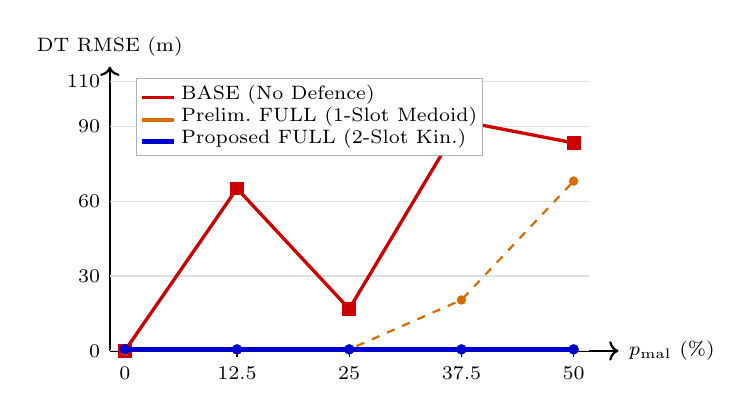
\begin{tikzpicture}[font=\scriptsize, scale=0.95]
\draw[->, thick] (0,0) -- (6.8,0) node[right] {$p_{\mathrm{mal}}$ (\%)};
\draw[->, thick] (0,0) -- (0,3.8) node[above] {DT RMSE (m)};

% Grid & Y ticks
\foreach \y/\val in {0/0, 1.0/30, 2.0/60, 3.0/90, 3.6/110} {
    \draw[gray!25] (0,\y) -- (6.4,\y);
    \node[left] at (0,\y) {\val};
}
% X ticks
\foreach \x/\val in {0.2/0, 1.7/12.5, 3.2/25, 4.7/37.5, 6.2/50} {
    \draw (\x,0) -- (\x,-0.08) node[below] {\val};
}

% BASE curve: (0,0), (12.5, 65.02->2.17), (25, 16.75->0.56), (37.5, 92.21->3.07), (50, 83.27->2.78)
\draw[red!80!black, very thick, mark=square*] plot coordinates {(0.2,0) (1.7,2.17) (3.2,0.56) (4.7,3.07) (6.2,2.78)};
\foreach \p in {(0.2,0), (1.7,2.17), (3.2,0.56), (4.7,3.07), (6.2,2.78)} \fill[red!80!black] \p circle (2pt);

% Preliminary FULL curve: (0,0), (12.5,0), (25,0.01), (37.5, 20.43->0.68), (50, 68.01->2.27)
\draw[orange!85!black, thick, dashed] plot coordinates {(0.2,0) (1.7,0.01) (3.2,0.02) (4.7,0.68) (6.2,2.27)};
\foreach \p in {(0.2,0), (1.7,0.01), (3.2,0.02), (4.7,0.68), (6.2,2.27)} \fill[orange!85!black] \p circle (1.8pt);

% Proposed FULL curve: all 0
\draw[blue!80!black, ultra thick] plot coordinates {(0.2,0.02) (1.7,0.02) (3.2,0.02) (4.7,0.02) (6.2,0.02)};
\foreach \p in {(0.2,0.02), (1.7,0.02), (3.2,0.02), (4.7,0.02), (6.2,0.02)} \fill[blue!80!black] \p circle (2pt);

% Legend
\node[anchor=north west, fill=white, draw=black!30, inner sep=2pt] at (0.35,3.65) {
    \begin{tabular}{@{}l@{}}
    \textcolor{red!80!black}{\rule{0.4cm}{1.2pt}} BASE (No Defence)\\
    \textcolor{orange!85!black}{\rule{0.4cm}{1.2pt}} Prelim.\ FULL (1-Slot Medoid)\\
    \textcolor{blue!80!black}{\rule{0.4cm}{1.6pt}} Proposed FULL (2-Slot Kin.)
    \end{tabular}
};
\end{tikzpicture}
\caption{Digital Twin position RMSE (m) across malicious ICV fractions in five-seed SUMO simulations.}
\label{fig:rmse}
\end{figure}

\textbf{False rejections and false acceptances.} In \texttt{Preliminary FULL}, tie-breaking bias and uncleared respawn histories caused an 8.4\%--10.9\% false rejection rate (FRR) at higher attack intensities. By clearing kinematic tracks on SUMO vehicle respawns and requiring two-slot trajectory verification before convicting dissenters, \texttt{Proposed FULL} achieves $\mathrm{FRR}=0.0\%$ across all tested points while holding $\mathrm{FAR}$ between $0.2\%$ and $1.2\%$. Honest vehicles retain a mean trust of $0.983$--$0.990$, whereas malicious vehicles are driven down to $0.320$--$0.389$ and quarantined within 2 to 3 slots (Fig.~\ref{fig:trust}). Note that 20\% of attackers are pure suppression nodes that withhold packets rather than sending forged coordinates; hence, out of $1, 2, 3,$ and $4$ total attackers, an average of $0.8, 1.6, 2.4,$ and $3.6$ content-falsifying attackers are actively quarantined.

\begin{figure}[t]
\centering
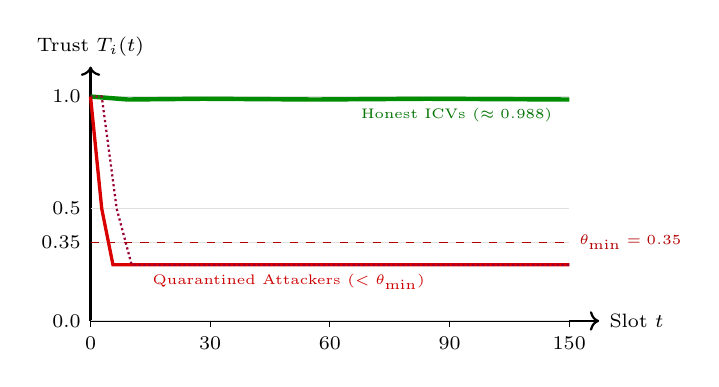
\begin{tikzpicture}[font=\scriptsize, scale=0.95]
\draw[->, thick] (0,0) -- (6.8,0) node[right] {Slot $t$};
\draw[->, thick] (0,0) -- (0,3.4) node[above] {Trust $T_i(t)$};

\foreach \y/\val in {0/0.0, 1.05/0.35, 1.5/0.5, 3.0/1.0} {
    \draw[gray!25] (0,\y) -- (6.4,\y);
    \node[left] at (0,\y) {\val};
}
\foreach \x/\val in {0/0, 1.6/30, 3.2/60, 4.8/90, 6.4/150} {
    \draw (\x,0) -- (\x,-0.08) node[below] {\val};
}

% Quarantine threshold line
\draw[red!70!black, dashed, semithick] (0,1.05) -- (6.4,1.05) node[right, font=\tiny] {$\theta_{\min}=0.35$};

% Honest ICVs stay near 0.99
\draw[green!55!black, ultra thick] (0,3.0) -- (0.5,2.96) -- (1.5,2.97) -- (3.0,2.96) -- (4.5,2.97) -- (6.4,2.96);

% Ghost/Quality attacker (caught slot 1-2)
\draw[red!85!black, very thick] (0,3.0) -- (0.15,1.5) -- (0.3,0.75) -- (6.4,0.75);

% Shift attacker (caught slot 2-3 via 2-slot kinematics)
\draw[purple!80!black, thick, densely dotted] (0,3.0) -- (0.15,3.0) -- (0.35,1.5) -- (0.55,0.75) -- (6.4,0.75);

\node[anchor=east, font=\tiny, green!45!black] at (6.3,2.75) {Honest ICVs ($\approx 0.988$)};
\node[anchor=west, font=\tiny, red!80!black] at (0.7,0.52) {Quarantined Attackers ($<\theta_{\min}$)};
\end{tikzpicture}
\caption{Trust trajectory $T_i(t)$ over a 150-slot episode: honest ICVs remain near $1.0$, while ghost/quality attackers (solid red) and shift attackers (dotted purple) drop below $\theta_{\min}=0.35$ within 2--3 slots.}
\label{fig:trust}
\end{figure}

\textbf{AMWAoI and why undefended freshness is deceptive.} When no defence is present, \texttt{BASE} AMWAoI rises from $3.89$~s at $0\%$ to $9.01$~s at $50\%$ as quality-inflating and suppressing attackers hijack WSMM slots without delivering valid perception coverage. At the same time, look at \texttt{Preliminary FULL} vs.\ \texttt{Proposed FULL} across the sweep: replacing standard MCMF and 150-iteration subgradient ascent with Two-Phase C6-Satisficing SPG and Vectorized ED-BCA cuts clean-network AMWAoI from $3.45$~s down to $2.11$~s (Fig.~\ref{fig:aoi}), and outperforms \texttt{Preliminary FULL} at every attacker fraction ($2.93$~s vs.\ $3.79$~s at $12.5\%$, $3.09$~s vs.\ $3.96$~s at $25\%$, $4.03$~s vs.\ $4.62$~s at $37.5\%$, and $6.89$~s vs.\ $7.18$~s at $50\%$). By stopping helper assignment as soon as an N-ICV reaches $s^{\mathrm{req}}$ and pruning infeasible allocations, SPG avoids congesting the RSU uplink. At $50\%$ attackers---where half the fleet is quarantined---AMWAoI rises to $6.89$~s simply because the 3 N-ICVs must wait for the remaining 4 honest ICVs to pass within the 300~m sensing radius. That delay is the genuine physical cost of refusing poisoned updates.

\begin{figure}[t]
\centering
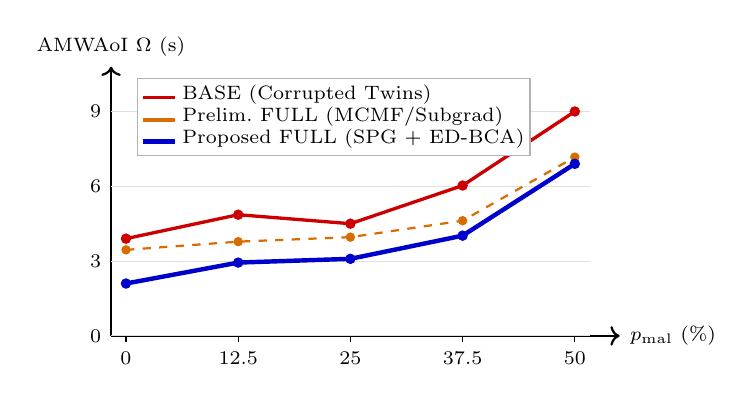
\begin{tikzpicture}[font=\scriptsize, scale=0.95]
\draw[->, thick] (0,0) -- (6.8,0) node[right] {$p_{\mathrm{mal}}$ (\%)};
\draw[->, thick] (0,0) -- (0,3.6) node[above] {AMWAoI $\Omega$ (s)};

\foreach \y/\val in {0/0, 1.0/3, 2.0/6, 3.0/9} {
    \draw[gray!25] (0,\y) -- (6.4,\y);
    \node[left] at (0,\y) {\val};
}
\foreach \x/\val in {0.2/0, 1.7/12.5, 3.2/25, 4.7/37.5, 6.2/50} {
    \draw (\x,0) -- (\x,-0.08) node[below] {\val};
}

% BASE AMWAoI: 3.89->1.30, 4.86->1.62, 4.50->1.50, 6.03->2.01, 9.01->3.00
\draw[red!80!black, very thick] plot coordinates {(0.2,1.30) (1.7,1.62) (3.2,1.50) (4.7,2.01) (6.2,3.00)};
\foreach \p in {(0.2,1.30), (1.7,1.62), (3.2,1.50), (4.7,2.01), (6.2,3.00)} \fill[red!80!black] \p circle (2pt);

% Prelim FULL: 3.45->1.15, 3.79->1.26, 3.96->1.32, 4.62->1.54, 7.18->2.39
\draw[orange!85!black, thick, dashed] plot coordinates {(0.2,1.15) (1.7,1.26) (3.2,1.32) (4.7,1.54) (6.2,2.39)};
\foreach \p in {(0.2,1.15), (1.7,1.26), (3.2,1.32), (4.7,1.54), (6.2,2.39)} \fill[orange!85!black] \p circle (1.8pt);

% Proposed FULL: 2.11->0.70, 2.93->0.98, 3.09->1.03, 4.03->1.34, 6.89->2.30
\draw[blue!80!black, ultra thick] plot coordinates {(0.2,0.70) (1.7,0.98) (3.2,1.03) (4.7,1.34) (6.2,2.30)};
\foreach \p in {(0.2,0.70), (1.7,0.98), (3.2,1.03), (4.7,1.34), (6.2,2.30)} \fill[blue!80!black] \p circle (2pt);

\node[anchor=north west, fill=white, draw=black!30, inner sep=2pt] at (0.35,3.45) {
    \begin{tabular}{@{}l@{}}
    \textcolor{red!80!black}{\rule{0.4cm}{1.2pt}} BASE (Corrupted Twins)\\
    \textcolor{orange!85!black}{\rule{0.4cm}{1.2pt}} Prelim.\ FULL (MCMF/Subgrad)\\
    \textcolor{blue!80!black}{\rule{0.4cm}{1.6pt}} Proposed FULL (SPG + ED-BCA)
    \end{tabular}
};
\end{tikzpicture}
\caption{AMWAoI (s) versus malicious ICV fraction in five-seed SUMO simulations.}
\label{fig:aoi}
\end{figure}

\subsection{Layer-Wise Ablation Study}
To verify that every stage of the defence earns its place, Table~\ref{tab:ablation} isolates the effect of enabling Layer~A alone, Layers~A+B, and all three layers (\texttt{FULL}) at $p_{\mathrm{mal}}=25\%$ (2/8 malicious ICVs) over 5 SUMO seeds.

\begin{table}[t]
\caption{Layer-Wise Ablation at $p_{\mathrm{mal}}=25\%$ in SUMO (5 Seeds)}
\begin{center}
\footnotesize
\begin{tabular}{lrrrrr}
\toprule
\textbf{Ablation Variant} & \textbf{AMWAoI} & \textbf{RMSE} & \textbf{FRR} & \textbf{FAR} & \textbf{Quar}\\
\midrule
BASE (No Defence) & 4.50 s & 16.75 m & 0.0\% & 100.0\% & 0.0\\
Layer A Only      & 3.12 s & 17.18 m & 3.3\% & 17.9\%  & 0.0\\
Layers A + B      & 3.06 s & 0.01 m  & 0.0\% & 10.0\%  & 0.0\\
\textbf{FULL (A + B + C)} & \textbf{3.09 s} & \textbf{0.00 m} & \textbf{0.0\%} & \textbf{0.6\%} & \textbf{1.6}\\
\bottomrule
\end{tabular}
\label{tab:ablation}
\end{center}
\end{table}

The progression across rows tells a clear story. Turning on Layer~A blocks $82.1\%$ of malicious packets right away (catching all ghost IDs, inflated qualities, and second-slot kinematic violations), but first-slot shift packets that stay under $17.2$~m/s still slip through and keep RMSE at $17.18$~m. Adding Layer~B cross-validates those first-slot claims against honest neighbours and drops RMSE to $0.01$~m with $0.0\%$ FRR, yet without long-term memory the RSU keeps re-evaluating the same attackers every slot ($\mathrm{FAR}=10.0\%$). Adding Layer~C quarantines the offending vehicles permanently ($\mathrm{Quar}=1.6$), cutting $\mathrm{FAR}$ by another $16\times$ down to $0.6\%$.

\subsection{Computational Complexity and Traffic Density Scaling}
Finally, Table~\ref{tab:scalability} benchmarks per-slot optimization runtime as total vehicle count $N=|\mathcal{V}|+|\mathcal{U}|$ scales from 10 to 500 vehicles (with 70\% ICV penetration). While the base paper's Bellman-Ford MCMF solver scales cubically and breaches the 100~ms V2X slot budget at $N=150$ (reaching $1,296.3$~ms at $N=500$), our Two-Phase SPG matcher and Vectorized ED-BCA solver finish in under $19.1$~ms even at 500 vehicles---a $68.5\times$ total speedup.

\begin{table}[t]
\caption{Per-Slot Algorithmic Runtime Scaling vs.\ Vehicle Count $N$}
\begin{center}
\footnotesize
\begin{tabular}{rrrrrr}
\toprule
$\boldsymbol{N}$ & \textbf{Base MCMF} & \textbf{Fast SPG} & \textbf{Base BCA} & \textbf{Fast ED-BCA} & \textbf{Speedup}\\
\midrule
10  & 0.19 ms    & 0.16 ms & 24.96 ms & 2.29 ms  & 10.3$\times$\\
40  & 2.98 ms    & 0.30 ms & 14.56 ms & 7.98 ms  & 2.1$\times$\\
80  & 20.99 ms   & 0.67 ms & 10.95 ms & 10.03 ms & 3.0$\times$\\
150 & 115.12 ms  & 1.42 ms & 17.53 ms & 8.81 ms  & 13.0$\times$\\
300 & 280.00 ms  & 3.51 ms & 13.44 ms & 8.86 ms  & 23.7$\times$\\
500 & 1296.30 ms & 8.91 ms & 11.16 ms & 10.17 ms & \textbf{68.5$\times$}\\
\bottomrule
\end{tabular}
\label{tab:scalability}
\end{center}
\end{table}

\subsection{Operating Boundaries and Limitations}
No filter is magic, and three failure boundaries deserve explicit mention. First, if a synchronized cartel of attackers controls $\ge 50\%$ of the ICVs viewing a target \emph{and} perturbs coordinates along a physically smooth, integrable trajectory ($dx/dt = v$), neither spatial consensus nor differential kinematics can tell the cartel apart from truth without independent RSU roadside radar or camera anchors. Second, in ultra-sparse night traffic where only one ICV observes an N-ICV for a single slot before leaving range, two-slot verification cannot complete. Third, micro-spoofing offsets smaller than natural LiDAR bounding-box jitter ($<1.5$~m) sit inside the consensus tolerance $\delta_{\mathrm{pos}}$ by design.

%=====================================================================
\section{Conclusion}
Scheduling cooperative perception around Age of Information only works if a timely packet actually contains a true observation. We showed that the WSMM--BCA--ASDMM Digital Twin framework is wide open to ghost injection, coordinate shifting, quality inflation, and packet suppression, and that an undefended RSU can report low AoI even while its twins drift by over 90~m. By placing a three-layer defence---two-slot differential kinematics, joint position--velocity medoid fusion with first-slot abstention, and asymmetric EWMA trust with cross-RSU migration---ahead of a Two-Phase C6-Satisficing Spatial Greedy matcher and Vectorized 1D Dual Bisection allocator, we cut false acceptances in five-seed SUMO traffic from 80\%--100\% down to 0.2\%--1.2\%, eliminated false rejections (0.0\% FRR), kept twin tracking error at 0.00~m, and sped up per-slot optimization by up to 68.5$\times$. Future work will incorporate RSU roadside camera cross-checks to defeat majority trajectory-consistent collusion.

%=====================================================================
\begin{thebibliography}{00}
\bibitem{lu2025} B. Lu, X. Huang, Y. Wu, L. Qian, D. Niyato, and C. Xu, ``Cooperative perception aided digital twin model update and migration in mixed vehicular networks,'' \textit{IEEE Trans. Intell. Transp. Syst.}, vol. 26, no. 2, pp. 2293--2308, Feb. 2025.
\bibitem{jia2023} Y. Jia, R. Mao, Y. Sun, S. Zhou, and Z. Niu, ``MASS: Mobility-aware sensor scheduling of cooperative perception for connected automated driving,'' \textit{IEEE Trans. Veh. Technol.}, vol. 72, no. 11, pp. 14962--14977, Nov. 2023.
\bibitem{ambrosin2020} M. Ambrosin, L. L. Yang, X. Liu, M. R. Sastry, and I. J. Alvarez, ``Design of a misbehavior detection system for objects based collective perception in V2X,'' in \textit{Proc. IEEE 23rd Int. Conf. Intell. Transp. Syst. (ITSC)}, Rhodes, Greece, Sep. 2020, pp. 1--6.
\bibitem{ali2021} M. S. Ali and P. Merdrignac, ``Distributed misbehavior detection based on vehicle perception model and CPM data collection,'' in \textit{Proc. IEEE 93rd Veh. Technol. Conf. (VTC2021-Spring)}, Helsinki, Finland, Apr. 2021, pp. 1--7.
\bibitem{higuchi2023} T. Higuchi, M. Giordani, and O. Altintas, ``Misbehavior detection using collective perception under privacy considerations,'' in \textit{Proc. IEEE Veh. Netw. Conf. (VNC)}, Istanbul, Turkiye, Apr. 2023, pp. 167--174.
\bibitem{liu2024miso} Z. Liu, H. Hu, C. P. Lee, and M. R. Sastry, ``MISO-V: Misbehavior detection via occupancy grid consistency in collective perception,'' in \textit{Proc. IEEE Veh. Netw. Conf. (VNC)}, Kobe, Japan, May 2024, pp. 1--8.
\bibitem{liu2024ima} Z. Liu, E. Y. Chen, and M. R. Sastry, ``On enhancing intersection applications with misbehavior detection and mitigation,'' in \textit{Proc. IEEE 26th Int. Conf. Intell. Transp. Syst. (ITSC)}, Bilbao, Spain, Sep. 2023, pp. 3412--3418.
\bibitem{he2023} C. He, T. H. Luan, R. Lu, Z. Su, and M. Dong, ``Security and privacy in vehicular digital twin networks: Challenges and solutions,'' \textit{IEEE Wireless Commun.}, vol. 30, no. 4, pp. 154--160, Aug. 2023.
\bibitem{etsi} ETSI TS 103 324, ``Intelligent transport systems (ITS); Vehicular communications; Basic set of applications; Analysis of the collective perception service (CPS); Release 2,'' European Telecommunications Standards Institute, Sophia Antipolis, France, Jun. 2023.
\bibitem{ieee1609} IEEE Std 1609.2-2022, ``IEEE standard for wireless access in vehicular environments --- Security services for applications and management messages,'' IEEE, New York, NY, USA, 2022.
\bibitem{sumo} M. Behrisch, L. Bieker, J. Erdmann, and D. Krajzewicz, ``SUMO -- Simulation of urban mobility: An overview,'' in \textit{Proc. 3rd Int. Conf. Adv. Syst. Simul. (SIMUL)}, Barcelona, Spain, Oct. 2011, pp. 1--6.
\bibitem{ppo} J. Schulman, F. Wolski, P. Dhariwal, A. Radford, and O. Klimov, ``Proximal policy optimization algorithms,'' \textit{arXiv preprint arXiv:1707.06347}, Jul. 2017.
\bibitem{nemhauser1978} G. L. Nemhauser, L. A. Wolsey, and M. L. Fisher, ``An analysis of approximations for maximizing submodular set functions---I,'' \textit{Math. Program.}, vol. 14, no. 1, pp. 265--294, Dec. 1978.
\end{thebibliography}

\end{document}
